\begin{frame}{Theory predictions}

\footnotesize

\begin{columns}[t]
\column{.5\textwidth}
1. Prediction for the production cross sections for different radial excitations of $\chi_b$ states:

$$
\frac{\sigma^{th}[2P,1S]}{\sigma^{th}[1P,1S]} = (0.29 \pm 0.01^{th} \pm 0.1^{br}) \Bigl| \frac{R'_{2P}}{R'_{1P}}\Bigr|^2, 
$$
\begin{itemize}
\item  $\sigma^{th}[nP,mS]$ ---  sum over the possible $\chi_b(nP)$ spin
states of the production cross section for that state multiplied by its
branching fraction for the $\Upsilon(mS)$ decay.
\item $R'_{nP} \sim 1$ --- derivative of the $\chi_b(nP)$ state wave function at the origin
\end{itemize}

\textbf{Predictions for this
ratio in the range between 0.14 and 0.4 have been obtained by using different
potential models.}

\column{.5\textwidth}
2. The $\sigma(\chi_{b2})/\sigma(\chi_{b1})$ ratio prediction
\resizebox{.9\textwidth}{!}{
\setlength{\unitlength}{1mm}
\begin{picture}(75,60)
%
 \put(0,0){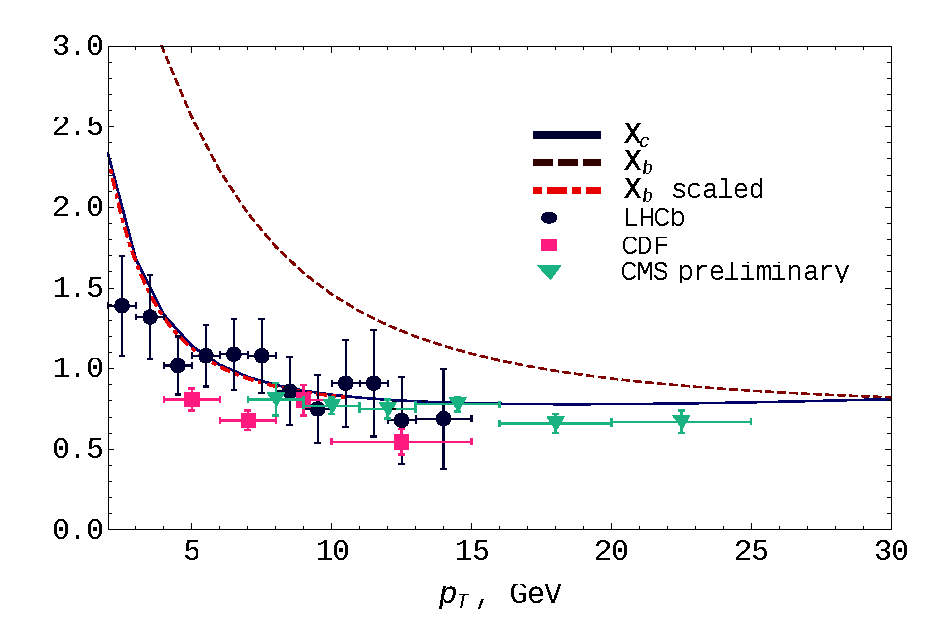
\includegraphics[width=75mm, height=60mm]{theory/ratio}}
 \put(-1,22){\begin{sideways}$\sigma({\chi_2})/\sigma({\chi_1}$)\end{sideways}}
\end{picture}
}
Transverse momentum distributions of the
$d\sigma\left[\chi_{2}\right]/d\sigma[\chi_{1}]$ ratio. Solid and dashed lines
stand for charmonium and bottomonium mesons. The dot-dashed line corresponds to
the rescaled bottomonium ratio.
\end{columns}
\end{frame}